%%%%%%%%%%%%%%%%%%%%%%%%%%%%%%%%%%%%%%%%%
% University/School Laboratory Report
% LaTeX Template
% Version 3.1 (25/3/14)
%
% This template has been downloaded from:
% http://www.LaTeXTemplates.com
%
% Original author:
% Linux and Unix Users Group at Virginia Tech Wiki 
% (https://vtluug.org/wiki/Example_LaTeX_chem_lab_report)
%
% License:
% CC BY-NC-SA 3.0 (http://creativecommons.org/licenses/by-nc-sa/3.0/)
%
%%%%%%%%%%%%%%%%%%%%%%%%%%%%%%%%%%%%%%%%%

%----------------------------------------------------------------------------------------
%	PACKAGES AND DOCUMENT CONFIGURATIONS
%----------------------------------------------------------------------------------------

\documentclass{report}
\usepackage[utf8]{inputenc}
\usepackage{siunitx} % Provides the \SI{}{} and \si{} command for typesetting SI units
\usepackage{graphicx} % Required for the inclusion of images
\usepackage{caption}
\usepackage{natbib} % Required to change bibliography style to APA
\usepackage{amsmath} % Required for some math elements 
\usepackage{amssymb}
%\usepackage{blindtext}
%\usepackage{tikz}
%\usetikzlibrary{matrix}
%%\setlength\parindent{0pt} % Removes all indentation from paragraphs
%\usepackage[framed]{matlab-prettifier}
%\definecolor{mygreen}{RGB}{28,172,0} % color values Red, Green, Blue
%\definecolor{mylilas}{RGB}{170,55,241}
%\usepackage{listings}
%\lstset{
%	style=Matlab-editor,
%	basicstyle         = \fontsize{8}{11}\ttfamily,
%	numberstyle       =\fontsize{8}{11}\ttfamily,
%	%backgroundcolor=\color{gray},
%	%mlshowsectionrules = true,
%	rangeprefix        = \%\ 
%}

\renewcommand{\labelenumi}{\alph{enumi}.} % Make numbering in the enumerate environment by letter rather than number (e.g. section 6)

%\usepackage{times} % Uncomment to use the Times New Roman font
%----------------------------------------------------------------------------------------
%	TITLE PAGE
%----------------------------------------------------------------------------------------
% Title Page
\title{Detection}
\author{Mauricio Caceres}
\date{13 février 2017}

%----------------------------------------------------------------------------------------
%	DOCUMENT INFORMATION
%----------------------------------------------------------------------------------------

\begin{document}
\begin{titlepage}
	\centering
	\vfill
{\bfseries\huge Detection et Estimation}
	\vfill
	{\bfseries\LARGE
		TP:\\
		Detection
		\\
		\vskip2cm

		Master SISEA\\
	
	}
	\vfill
	10 février 2017
	\vfill
	{\large Mauricio Caceres } \hfill  {\large Pierre-Samuel Garreau-Hamard}
	\vfill
	{\large Enseignant : Di Ge }
	\vfill
	
\includegraphics[width=9cm]{rennes} % also works with logo.pdf    
%	\vfill
%	
\includegraphics[width=6cm]{enssat} % also works with logo.pdf
	\vfill
	\vfill
\end{titlepage}


%\begin{center}
%\begin{tabular}{l r}
%Date Performed: & January 1, 2012 \\ % Date the experiment was performed
%Partners: & James Smith \\ % Partner names
%& Mary Smith \\
%Instructor: & Professor Smith % Instructor/supervisor
%\end{tabular}
%\end{center}


% If you wish to include an abstract, uncomment the lines below
% \begin{abstract}
% Abstract text
% \end{abstract}

%----------------------------------------------------------------------------------------
%	SECTION 1
%----------------------------------------------------------------------------------------
\chapter{Introduction}
\section{Objectif}



\section{Write the log likelihoood funciton $L(A,\phi)$ for a given observation vector}
\label{estimationProblem}

We have the signal 
\begin{equation}\label{key}
x(n) = A cos (2\pi f_0 n + \phi) + w(n)
\end{equation}

The non deterministic part of the signal is the noise. A White Gaussian noise with variance $\sigma ^2$, wich is common in many fields. So the log-likelihood function is evaluated in function of this noise with the next expression.
\begin{equation}\label{key}
w(n) = x(n) - A cos (2\pi f_0 n + \phi)
\end{equation}

\subsection{About the unit of $f_0$}

In the continous case the frequency belong to the reals numbers,
\begin{equation}\label{key}
w(n) = x(n) - A cos (2\pi f t + \phi)
\end{equation}
 but in the discrete case 

\begin{equation}\label{key}
t = nT_e = \frac{n}{f_e}
\end{equation}

\begin{equation}\label{key}
w(n) = x(n) - A cos (2\pi \frac{n}{f_e} f + \phi)
\end{equation}

Thus $\frac{f}{f_e} = f_0$ is dimensionless.
The Shannon condition must be accomplish

\begin{equation}\label{key}
f_e \geq 2f_{max}
\end{equation}

\begin{equation}\label{key}
0 \leq f_0 = \frac{f}{f_e} \leq 0.5
\end{equation}

We will chose an arbitrary value of $f_0$ respecting always the Shannon's Theorems




\begin{equation}\label{key}
w(n) = x(n) - A cos (2\pi f_0 n + \phi)
\end{equation}
The WGN distributions are iid so 
\begin{equation}\label{key}
P(w(n)|A,\theta ) = \prod_{n=0}^{N-1} P_w(w(n))
\end{equation}

So the log-likelihood function $L(A,\phi)$ is 

\begin{equation}\label{key}
L(A,\phi) = log P(w(n)|A,\theta )
\end{equation}

\begin{equation}\label{key}
L(A,\phi) = log \prod_{n=0}^{N-1} P_w(w(n))
\end{equation}

\begin{equation}\label{key}
L(A,\phi) = \sum_{n=0}^{N-1} log P_w(w(n))
\end{equation}

\begin{equation}\label{key}
L(A,\phi) = \sum_{n=0}^{N-1} log(\frac{1}{\sigma \sqrt{2\pi}}\exp{[-1/2(\frac{x(n) - A cos (2\pi f_0 n + \phi)-\mu}{\sigma})^2]}
\end{equation}

\begin{equation}\label{key}
L(A,\phi) = \sum_{n=0}^{N-1} B + ({[-1/2(\frac{x(n) - A cos (2\pi f_0 n + \phi)-\mu}{\sigma})^2]}a
\end{equation}

\section{Show the expression of each maximum likelihood estimators }
The derivate of the maximun likelihood function L respect to 
each parameter is
\begin{equation}\label{key}
\frac{\partial L(A,\phi)}{\partial A} = \sum_{n=0}^{N-1} (\frac{x(n) - A cos (2\pi f_0 n + \phi)-\mu}{\sigma})(\frac{cos(2\pi f_0 n +\phi}{\sigma})
\end{equation}

\begin{equation}\label{key}
\frac{\partial L(A,\phi)}{\partial \phi} = \sum_{n=0}^{N-1} - (\frac{x(n) - A cos (2\pi f_0 n + \phi)-\mu}{\sigma})(\frac{Asin(2\pi f_0 n +\phi}{\sigma})
\end{equation}

Taking the derivate respecto to the parameter $\phi $ and being equal to zero to find the maximum
\begin{equation}\label{key}
\frac{\partial L(A,\phi)}{\partial \phi} = 0 = \sum_{n=0}^{N-1} - (\frac{Ax(n)sin(2\pi f_0 n +\phi)}{\sigma^2}-\frac{A^2cos(2\pi f_0 n +\phi)sin(2\pi f_0 n +\phi)}{\sigma^2}) = 0
\end{equation}


\begin{equation}\label{key}
\frac{\partial L(A,\phi)}{\partial \phi} = 0 = \sum_{n=0}^{N-1} - (\frac{Ax(n)sin(2\pi f_0 n +\phi)}{\sigma^2}-\frac{A^2cos(2\pi f_0 n +\pi)sin(2\pi f_0 n +\phi)}{\sigma^2}) = 0
\end{equation}

\begin{equation}\label{key}
\frac{\partial L(A,\phi)}{\partial \phi} = 0 = \frac{A}{\sigma^2} \sum_{n=0}^{N-1} - (\frac{Ax(n)sin(2\pi f_0 n +\phi)-A^2cos(2\phi f_0 n +\pi)sin(2\phi f_0 n +\phi)}{\sigma^2}) = 0
\end{equation}


\begin{equation}\label{key}
\frac{\partial L(A,\phi)}{\partial \phi} = 0 = \sum_{n=0}^{N-1}(x(n)sin(2\pi f_0 n +\phi) - Acos(2\pi f_0 n +\pi))sin(2\phi f_0 n +\phi)) = 0
\end{equation}


\begin{equation}\label{key}
\frac{\partial L(A,\phi)}{\partial \phi} = 0 = \sum_{n=0}^{N-1}(x(n)sin(2\pi f_0 n +\phi) - A\sum_{n=0}^{N-1}cos(2\pi f_0 n +\phi)sin(2\pi f_0 n +\phi)) = 0
\end{equation}

Using the entity 

\begin{equation}\label{entitycossin}
\sum_{n=0}^{N-1}cos(2\pi f_0 n +\phi)sin(2\pi f_0 n +\phi)) \approx 0
\end{equation}

\begin{equation}\label{key}
\frac{\partial L(A,\phi)}{\partial \phi} = 0 = \sum_{n=0}^{N-1}(x(n)sin(2\pi f_0 n +\phi) = 0
\end{equation}

Developing the sum of angles

%\begin{equation}\label{key}
\begin{gather*} 
\frac{\partial L(A,\phi)}{\partial \phi} = 0 = \sum_{n=0}^{N-1}x(n)(sin(2\pi f_0 n +\phi)cos(2\pi f_0 n +\phi) + cos(2\pi f_0 n +\phi)sin(2\pi f_0 n +\phi)) = 0
\end{gather*}
%\end{equation}

\begin{equation}\label{key}
\frac{\partial L(A,\phi)}{\partial \phi} = 0 = \sum_{n=0}^{N-1}x(n)(sin(2\pi f_0 n +\phi)cos(\phi) = - \sum_{n=0}^{N-1}x(n)cos(2\pi f_0 n +\phi)sin(\phi)) 
\end{equation}



\begin{equation}\label{key}
\frac{\sum_{n=0}^{N-1}x(n)sin(2\pi f_0 n)}{\sum_{n=0}^{N-1}x(n)cos(2\pi f_0 n )} = \frac{sin(\phi )}{cos(\phi)} = tg(\phi)
\end{equation}

We verify the expresion

\begin{equation}\label{key}
\hat{\Phi}_{ML} = arctg(-\frac{\sum_{n=0}^{N-1}x(n)sin(2\pi f_0 n)}{\sum_{n=0}^{N-1}x(n)cos(2\pi f_0 n )})
\end{equation}


So for the expression of the estimator of A we have taking the
eq 1.15 and being equal to zero

\begin{equation}\label{key}
\frac{\partial L(A,\phi)}{\partial A} = \sum_{n=0}^{N-1} (\frac{x(n) - A cos (2\pi f_0 n + \phi)-\mu}{\sigma})(\frac{cos(2\pi f_0 n +\phi}{\sigma}) = 0
\end{equation}

\begin{equation}\label{key}
\sum_{n=0}^{N-1}x(n)cos(2\pi f_0 n + \phi) = A\sum_{n=0}^{N-1}cos^2(2\pi f_0 n + \phi)
\end{equation}

And more directly we obtain the next expression

\begin{equation}\label{key}
\hat{A} = \frac{\sum_{n=0}^{N-1}x(n)cos(2\pi f_0 n + \phi)}{\sum_{n=0}^{N-1}cos^2(2\pi f_0 n + \phi)}
\end{equation}











\section{Give the condition under which $ \hat{\Phi}_ML \approx \phi $ 
different from $ E|\hat{\Phi}_ML| \approx \phi $ }
\label{sec:condition}


Condition pour $\hat{\Phi}_{ML} \approx \Phi$

\begin{equation}\label{key}
tan(\hat{\Phi}_{ML} ) \approx tan(\Phi)
\end{equation}



\begin{gather*}
\frac{\sum_{n=0}^{N-1}x(n)sin(2\pi f_0n+\phi)}{\sum_{n=0}^{N-1}x(n)cos(2\pi f_0n+\phi)} = \\
\frac{\sum_{n=0}^{N-1}Acos(2\pi f_0n+\phi)+w(n)sin(2\pi f_0n+\phi)}{\sum_{n=0}^{N-1}Acos(2\pi f_0n+\phi)+w(n)cos(2\pi f_0n+\phi)}
\end{gather*}


\begin{gather*}
\frac{\sum_{n=0}^{N-1}x(n)sin(2\pi f_0n+\phi)}{\sum_{n=0}^{N-1}x(n)cos(2\pi f_0n+\phi)} = \\
\frac{\sum_{n=0}^{N-1}Acos(2\pi f_0n+\phi)+w(n)sin(2\pi f_0n+\phi)}{\sum_{n=0}^{N-1}Acos(2\pi f_0n+\phi)+w(n)cos(2\pi f_0n+\phi)}
\end{gather*}



\begin{gather*}
\frac{AN/2 sin(\phi)\sum_{n=0}^{N-1}w(n)sin(2\pi f_0n)}{AN/2 sin(\phi)\sum_{n=0}^{N-1}w(n)cos(2\pi f_0n)} \approx tan(\Phi)
\end{gather*}

This term will be next to $tan(\Phi)$ when 

\begin{equation}\label{key}
\sum_{n=0}^{N-1}|w(n)sin(2\pi f_0n)|<<|AN/2 sin(\phi)|
\end{equation}

and when we have 
\begin{equation}\label{key}
\sum_{n=0}^{N-1}|w(n)cos(2\pi f_0n)|<<|AN/2 cos(\phi)|
\end{equation}

The noise have a normal distribution so the sum of noise have the next distribution

\begin{equation}\label{key}
\sum_{n=0}^{N-1}|w(n)sin(2\pi f_0n)|\sim \textit{N}(0,N\sigma^2/2)
\end{equation}


We take a probabilité of 3$\sigma$
\begin{gather*}\label{key}
3\sqrt{\sigma^2 N/2} = 3\sqrt{N/2}\sigma << AN/2 sin(\phi)
\end{gather*}
%3 << \frac{A\sqrt{N}}{\sigma}sin(\phi)
For larges values of N $ \hat{\Phi}_ML \approx \phi $

We cans observe that the parameters A, $ \sigma $ and N can modified
the estimator properties.

The ratio $ \frac{A^2}{\sigma^2} $ represent the RSB %SEARCH THIS DEFINITION


It's clear that it's not the same when $ E|\hat{\Phi}_ML| \approx \phi $  where 
the mean of the distribution of values of the estimator is close to the true 
value of $ \phi $ to the next expresion $ \hat{\Phi}_{ML} \approx \phi $ that 
means that the values of the estimator are always close to the true value of $ 
\phi $ (the distribution is more strait around the true value)

To know what are the contraints around $f_0$

\begin{gather*}
sen(\alpha)cos(\alpha) = 1/2 sin(2\alpha)\\
cos^2(\alpha) = \frac{1+cos(2\alpha)}{2}\\
sin^2(\alpha) = \frac{1-cos(2\alpha)}{2}
\end{gather*}

In the entities of the copy, we obtain 

\begin{equation}\label{key}
\sum_{n=0}^{N-1}cos(4\pi f_0 n) \approx 0
\end{equation}

\begin{equation}\label{key}
\sum_{n=0}^{N-1}sin(4\pi f_0 n) \approx 0
\end{equation}

And the last entity 

\begin{equation}\label{key}
\sum_{n=0}^{N-1}(e^{j4\pi f_0n}) \approx 0
\end{equation}


With $\phi = 4\pi f_0$ and $f_0 =(0,1/2) $ these values not estan allowed because they violate the theorem of shannon



We have to exclude the values
$ \phi = 4\pi fo  $
$ \phi = 2\pi $
$ \phi = 0 $. The values corresponding to the axes


\section{Verify that the maximun-likehood estimator of the amplitude is 
	unbiased if $ \phi =  \hat{\Phi}_{ML} $}

The estimator is unbiased if $ E[\hat{A}] = A $ thus

\begin{equation}
E[\frac{2}{N}\sum_{n=0}^{N-1}x(n)cos(2\pi f_0 n + \hat{\Phi}_{ML})]
\end{equation}

with $ \phi =  \hat{\Phi}_{ML} $

\begin{equation}
\frac{2}{N}E[\sum_{n=0}^{N-1}Acos^2(2\pi f_0 n + \phi)]+E[w(n)]cos(2\pi f_0 n + 
\phi) = A
\end{equation}

And $ E[w(n)=0 $


\begin{equation}
\frac{2}{N}E[\sum_{n=0}^{N-1}Acos^2(2\pi f_0 n] = A
\end{equation}

\begin{equation}
\frac{2}{N} A \frac{N}{2} = A
\end{equation}

And we verify that the estimator is unbiased
\begin{equation}
E[\hat{A}] = A
\end{equation}




\section{To compute the term of Fisher Matrix}
Making the derivation to the other parameter $ \phi $

\begin{gather*}\label{key}
\frac{\partial^2 L(A,\phi)}{\partial \phi^2} = \sum_{n=0}^{N-1} - 
(\frac{Asin(2\pi f_0 n +\phi)}{\sigma}) (\frac{Asin(2\pi f_0 n 
	+\phi)}{\sigma})+\\
\sum_{n=0}^{N-1} - (\frac{x(n)-Acos(2\pi f_0 n +\phi)}{\sigma}) 
(\frac{Acos(2\pi f_0 n +\phi)}{\sigma})
\end{gather*}


\begin{gather*}\label{key}
\frac{\partial^2 L(A,\phi)}{\partial \phi^2} = \sum_{n=0}^{N-1} - 
(\frac{A^2sin^2(2\pi f_0 n +\phi)}{\sigma^2})+\\
\sum_{n=0}^{N-1} - (\frac{x(n)Acos(2\pi f_0 n +\phi)-A^2cos^2(2\pi f_0 n 
	+\phi)}{\sigma^2})
\end{gather*}


\begin{gather*}\label{key}
\frac{\partial^2 L(A,\phi)}{\partial \phi^2} = \sum_{n=0}^{N-1} - 
(\frac{A^2sin^2(2\pi f_0 n +\phi)}{\sigma^2})+\\
\sum_{n=0}^{N-1} (\frac{w(n)}{\sigma^2})
\end{gather*}

\begin{equation}\label{key}
-\sum_{n=0}^{N-1} E[\frac{\partial^2 L(A,\phi)}{\partial \phi^2}] = 
\sum_{n=0}^{N-1}\frac{A^2sin^2(2\pi f_0 n +\phi)}{\sigma^2}
\end{equation}

We obtain one of the terms of the fisher information matrix

\begin{equation}\label{key}
-\sum_{n=0}^{N-1} E[\frac{\partial^2 L(A,\phi)}{\partial \phi^2}] = 
\frac{A^2N}{\sigma^2 2}
\end{equation} 

The cross derivation to the other parameter

\begin{gather*}\label{key}
[\frac{\partial^2 L(A,\phi)}{\partial \phi \partial A}] = -\sum_{n=0}^{N-1} 
\frac{- cos(2\pi f_0 n +\phi)}{\sigma} \frac{Asin(2\pi f_0 n +\phi)}{\sigma} 
\\  + \sum_{n=0}^{N-1} - \frac{x(n)- Acos(2\pi f_0 n +\phi)}{\sigma} 
\frac{sin(2\pi f_0 n +\phi)}{\sigma} = [\frac{\partial^2 L(A,\phi)}{ \partial 
	A\partial \phi}] 
\end{gather*}

\begin{equation}\label{key}
-\sum_{n=0}^{N-1} E[\frac{\partial^2 L(A,\phi)}{\partial \phi \partial A}] = 
-\sum_{n=0}^{N-1} \frac{- cos(2\pi f_0 n +\phi)}{\sigma} \frac{Asin(2\pi f_0 n 
	+\phi)}{\sigma}
\end{equation} 

Using the simplification in equation \ref{entitycossin} we will obtain a 
symmetric matrix

\begin{equation}\label{key}
-\sum_{n=0}^{N-1} E[\frac{\partial^2 L(A,\phi)}{\partial \phi \partial A}] = 0
\end{equation} 

The derivation respect the parameter A

\begin{equation}
\frac{\partial^2 L(A,\phi)}{\partial A ^2} = -\sum_{n=0}^{N-1} 
(\frac{-cos(2\pi f_0 n + \phi)}{\sigma})(\frac{cos(2\pi f_0n + \phi)}{\sigma})
\end{equation}



\begin{equation}
\frac{\partial^2 L(A,\phi)}{\partial A ^2} = \frac{-1}{\sigma}-\sum_{n=0}^{N-1} 
cos^2(2\pi f_0 n + \phi) = \frac{-N}{2\sigma}
\end{equation}

The calculation of the expeted value for the fisher information matrix is

\begin{equation}
-\sum_{n=0}^{N-1} E[\frac{\partial^2 L(A,\phi)}{\partial A^2}] = {N}{2\sigma}
\end{equation} 


The fisher information matrix is 


\begin{equation}
J(A,\phi)=\begin{pmatrix}
\frac{A^2N}{\sigma^2 2} & 0 \\ 
0 & \frac{N}{2\sigma^2}
\end{pmatrix} 
\end{equation}

The Cramer-Rao lower bound in the unbiased case is 

\begin{equation}
CRLB = J(A,\phi)^{-1} = =\begin{pmatrix}
\frac{\sigma^2 2}{A^2N} & 0 \\ 
0 & \frac{2\sigma^2}{N}
\end{pmatrix} 
\end{equation}




























%------------------------------------------------------------
%	SECTION 2
%------------------------------------------------------------
\chapter{Implementation in Matlab }




\section{Results}

We observe that the estimation error of A always converge to zero when the 
number of points used in the calculation is large enough (>1000). We cane deduce 
that the estimator of A is quite good, because we just have to add an offset to 
suppress the error.
But, for the estimation error of phi converge more easily, we see the values oscillate 
a bit but the error drops down of 0.005 with N = 1000 so the estimator is efficient.


\begin{figure}[h]
	\centering
	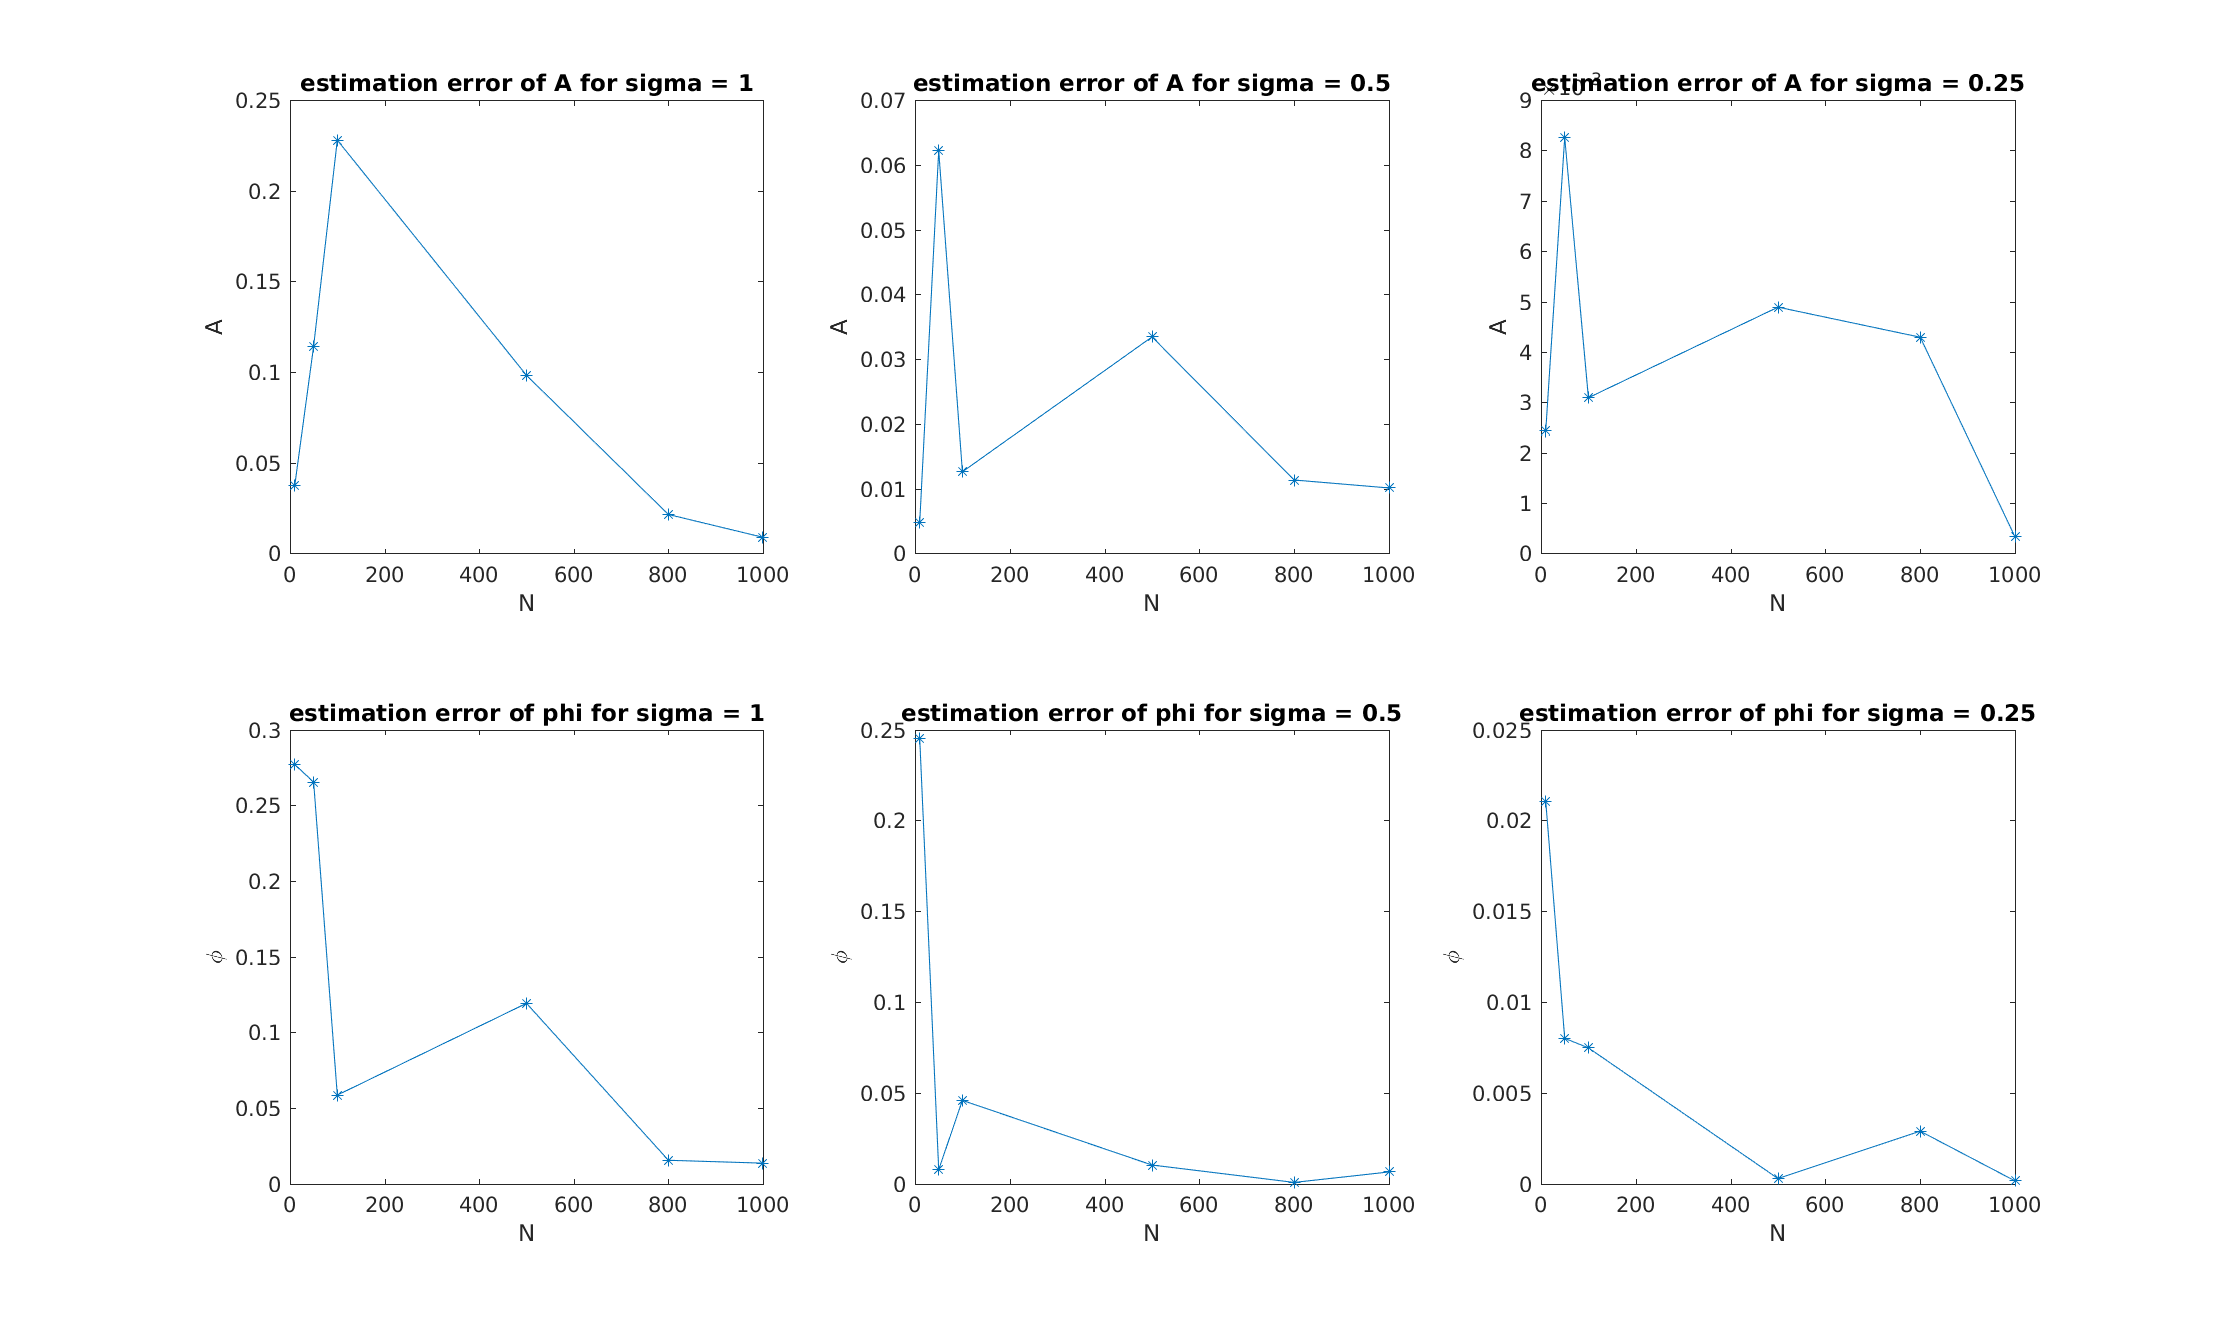
\includegraphics[width=\linewidth]{../1000_2}
	\caption{Curves for all the estimation cases, N = 1000 in the last iteration}
	\label{fig:10002}
\end{figure}

\begin{figure}[h]
	\centering
	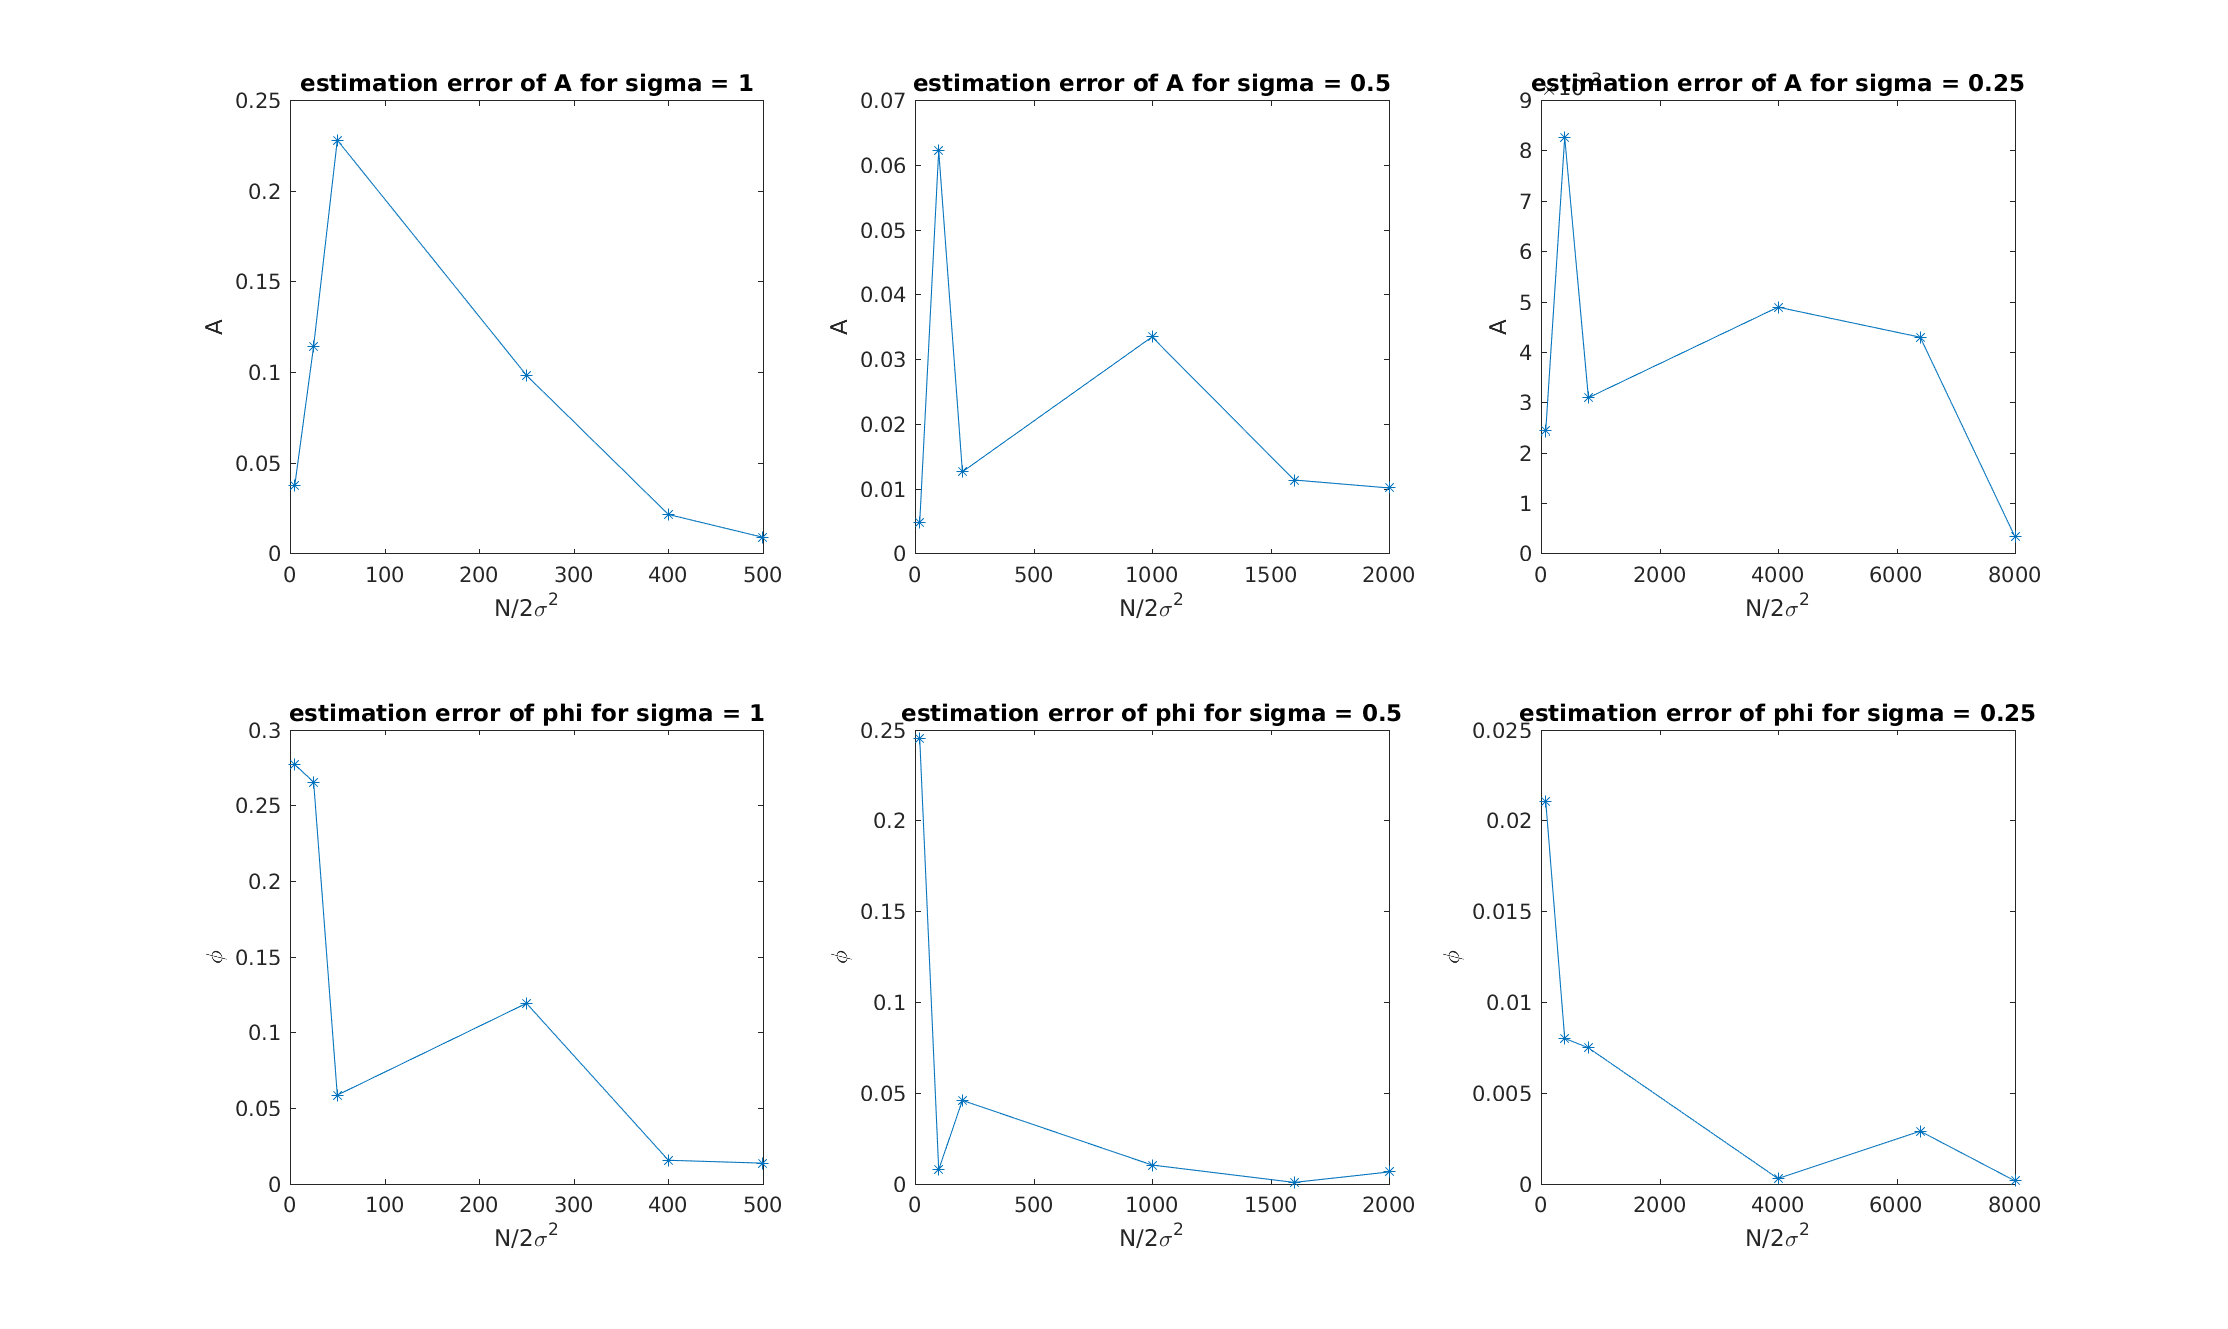
\includegraphics[width=\linewidth]{../1000_3}
	\caption{Curves for all the estimation cases in function of the Fisher information}
	\label{fig:10003}
\end{figure}


\begin{figure}[h]
	\centering
	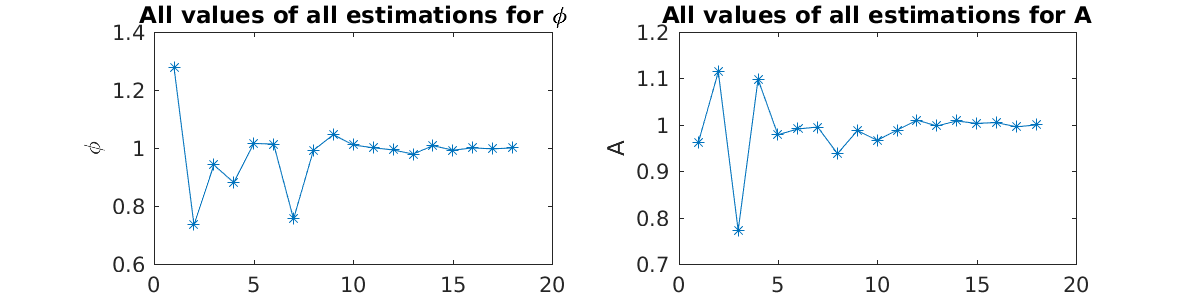
\includegraphics[width=0.7\linewidth]{../1000_4}
	\caption{Values for the estimations in each iteration}
	\label{fig:10004}
\end{figure}
We can see in the Fig \ref{fig:10004} all the estimations values. At each iteration the value 
oscillate around one arriving in the lastest iteration to acceptable value.


\subsection{Estimation with N = 2000}



We can state that for a value of N the error descends up to being an almost zero. 
With this we state that with this value of N = 200 our estimator one is the sufficiently
precise thing to estimate the real value.

It is correct also by the condition etablished in sec \ref{sec:condition} where it says 

Where it is said that increased the proportion $\frac{A\sqrt{N}}{\sigma}$ of someone of all the possible forms we will have a value of estimation much more reliable
\begin{figure}[h]
	\centering
	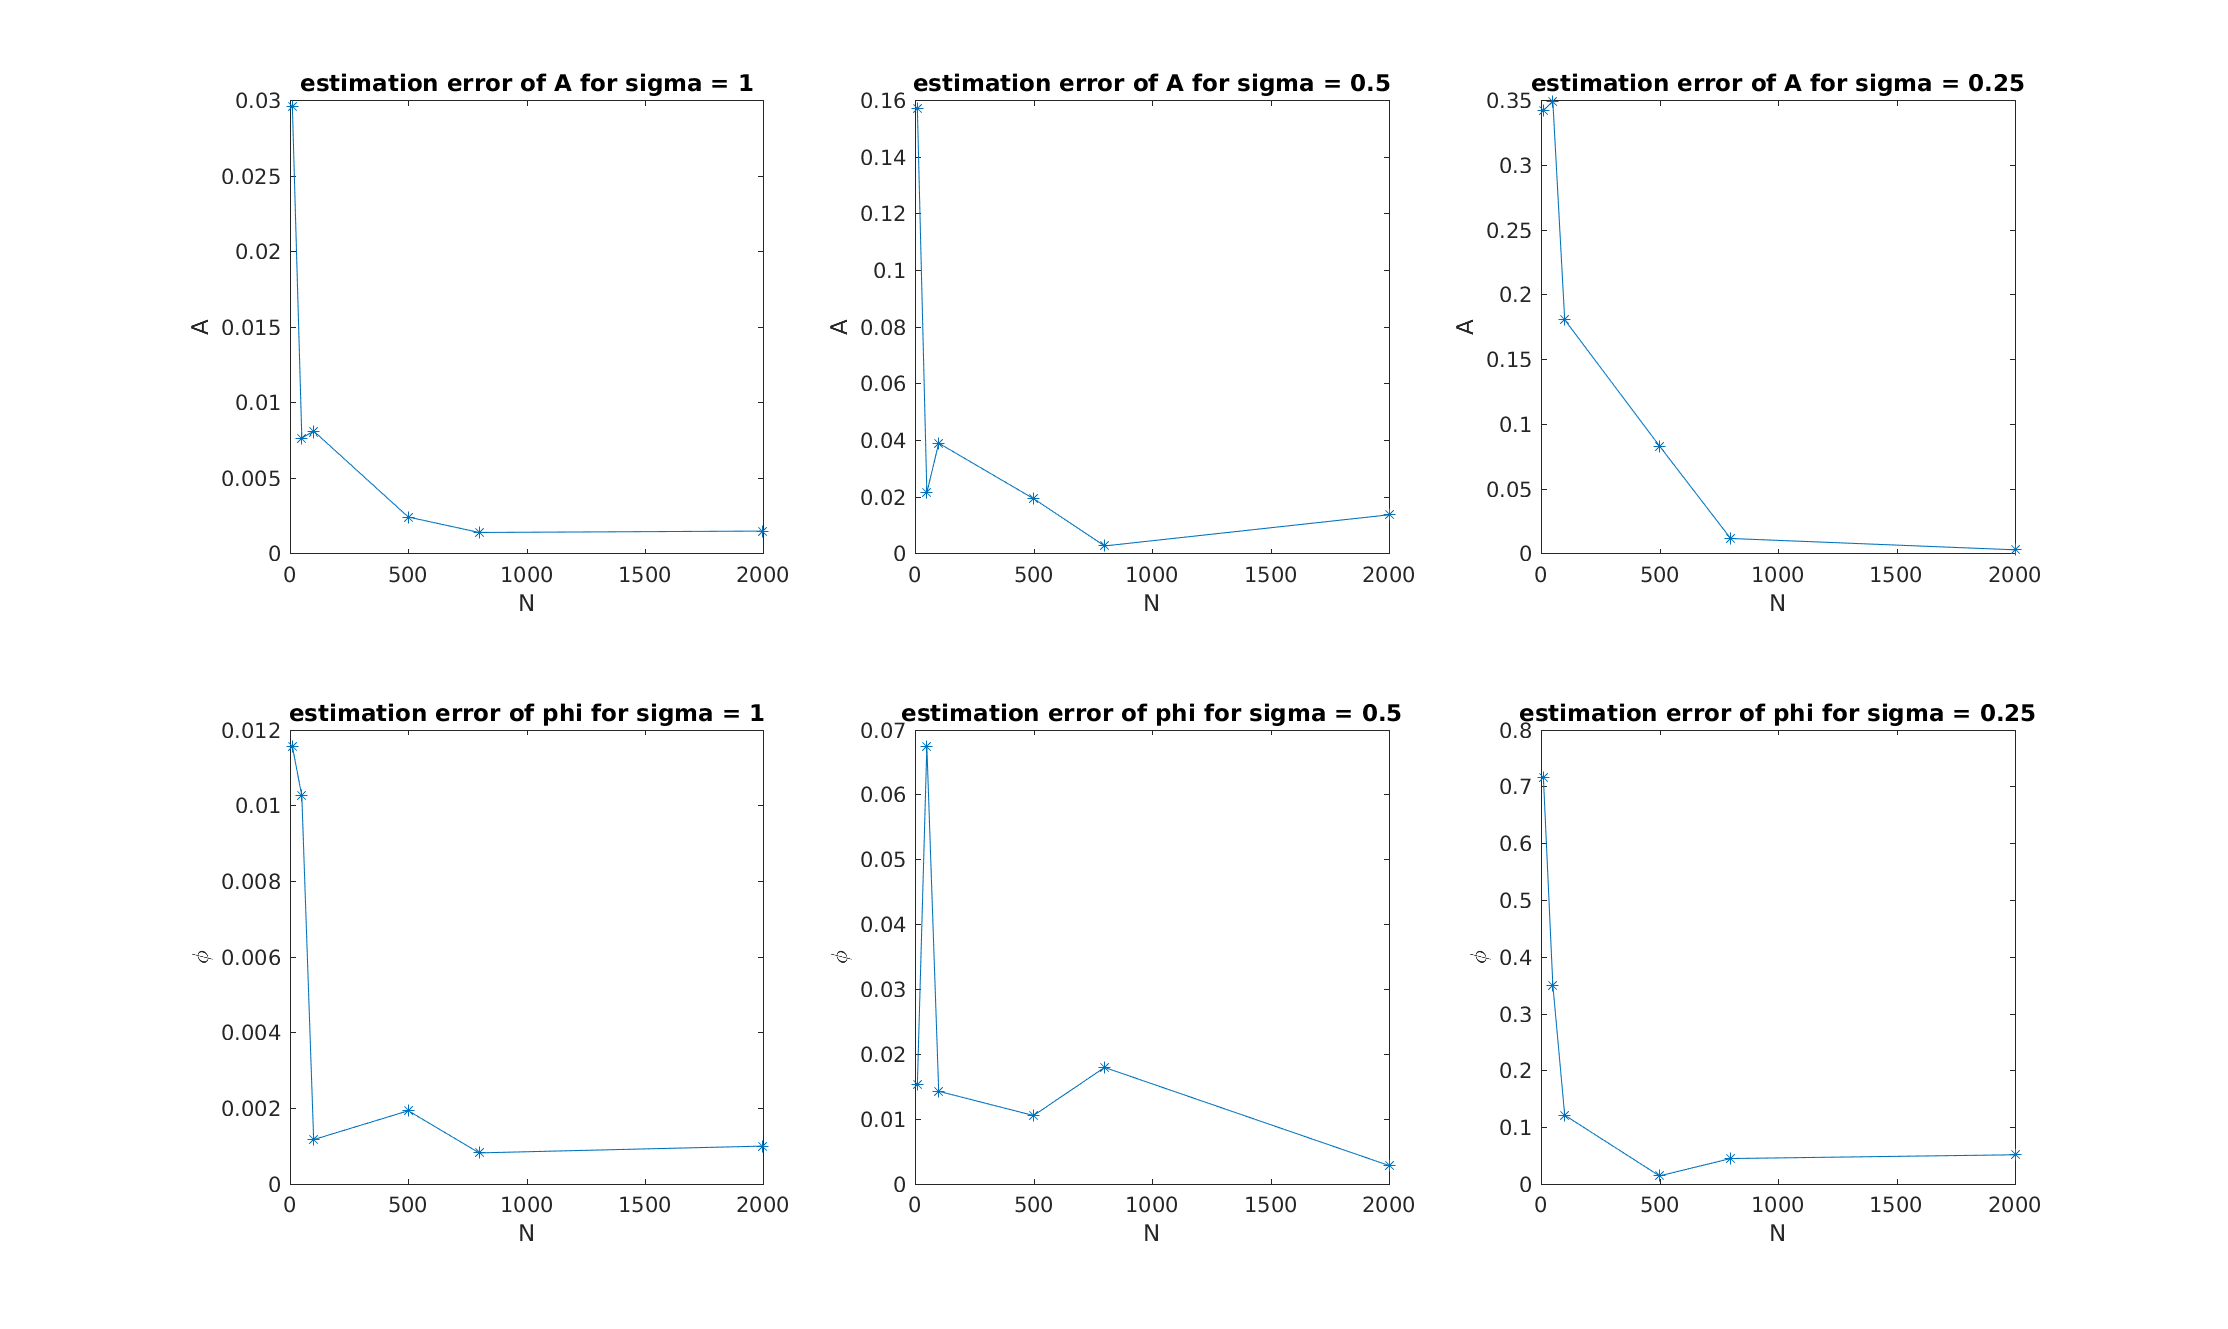
\includegraphics[width=\linewidth]{../2000_2}
	\caption{Curves for all the estimation cases}
	\label{fig:10002}
\end{figure}

%\begin{figure}[h]
%	\centering
%	
\includegraphics[width=\linewidth]{../2000_3}
%	\caption{Curves for all the estimation cases in function of the Fisher information}
%	\label{fig:10002}
%\end{figure}


%----------------------------------------------------------------------------------------
%	SECTION 3
%----------------------------------------------------------------------------------------

\newpage
\section{Conclusion}

We see across these exercises that the calculation of estimators and the execution of the simulations has coherence and respect the expected behavior. The results are satisfactory enough having estimator with a low enough error for values of N not so high and for the case in which N has a big value an almost void error is accomplished.\\
The evaluation with regard to all the parameters allows us to see in addition which is the influence of each one of them.
To see the curve corresponding to all the values of the estimator one gives us an idea of the dynamics of the calculation and since the values range about the expected value (one in our case).
The manual calculation and the mathematical demonstrations  for the expressions of the estimators ones showed us different tools that will allow us to understand that these mathematical tools are very useful and with a lot of applications.



%----------------------------------------------------------------------------------------
%	FIN
%----------------------------------------------------------------------------------------



\end{document}























